\chapter{Newton-Verfahren\label{chapter:newton}}
\lhead{Newton-Verfahren}
\rhead{}

\section{Nullstellen von Funktionen}
\rhead{Nullstellen von Funktionen}
\begin{figure}
\centering
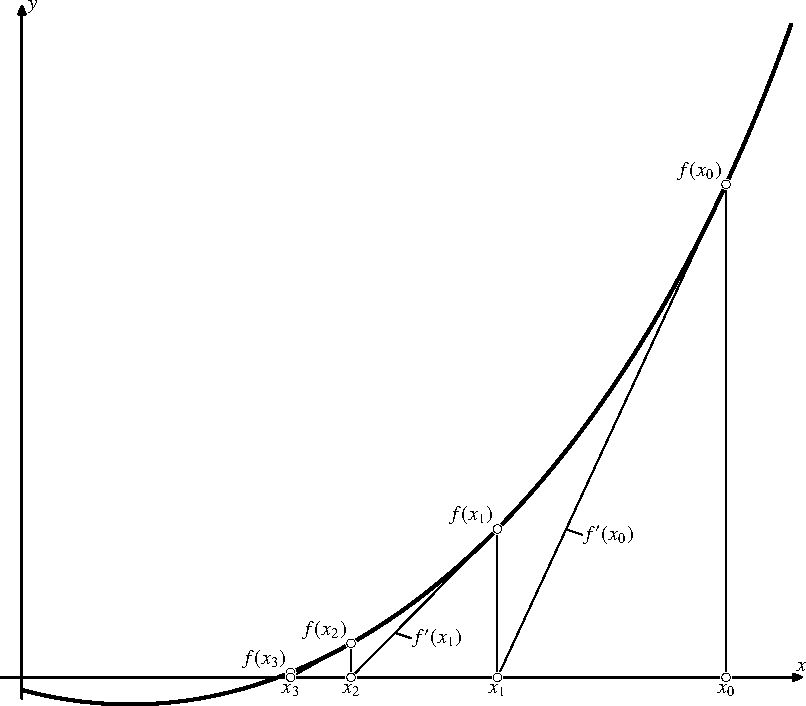
\includegraphics{chapters/images/randwert-2.pdf}
\caption{Bestimmung der Nullstelle einer Funktion $f(x)$ mit dem
Newton-Verfahren.
Die Approximation $x_{n+1}$ wird gefunden als Schnittpunkt der Tangente
im Punkt $(x_n,f(x_n))$ (mit Steigung $f'(x_n)$) mit der $x$-Achse.
\label{newton:graphik}}
\end{figure}
Das Ziel dieses Anhangs ist, die folgende Aufgabe numerisch zu l"osen:
\begin{aufgabe}
Gegeben ist eine differenzierbar Funktion
$f\colon\mathbb R\to\mathbb R:x\mapsto f(x)$
und eine Zahl $y$ im Wertebereich von $f$.
Finde $\hat{x}\in\mathbb R$ so, dass $f(\hat{x})=y$.
\end{aufgabe}
Im allgemeinen kann man nicht davon ausgehen, dass sich eine L"osung der
Gleichung $f(x)=y$ in geschlossener Form finden l"asst.
Nur einige wenige Klassen von Gleichungen haben L"osungsformeln dieser Art.
Wir beschr"anken uns daher auf das Problem, eine Approximation f"ur die
L"osung zu bestimmen.

Indem wir statt der Funktion $f(x)$ die Funktion $x\mapsto g(x)=f(x)-y$
betrachten, k"onnen wir die gesuchte Zahl $x$ auch als L"osung der
Gleichung $g(x)=0$ finden:
\begin{equation}
f(x)=y
\qquad\qquad
\Rightarrow
\qquad\qquad
g(x)=f(x)-y = 0.
\label{newton:reduktion}
\end{equation}
Es gen"ugt also, ein L"osungsverfahren zu entwickeln f"ur die Aufgabe
\begin{aufgabe}
Gegeben ist eine differenzierbar Funktion
$f\colon\mathbb R\to\mathbb R:x\mapsto f(x)$,
finde $\hat{x}\in\mathbb R$ so, dass $f(\hat{x})=0$.
\end{aufgabe}
Da wir nur eine numerische L"osung brauchen, versuchen wir sie dadurch
zu finden, dass wir eine Anfangssch"atzung $x_0$ wiederholt korrigieren,
bis der Fehler klein genug ist.
Es soll also eine Folge $x_0,x_1,x_2,\dots$ konstruiert werden, welche
gegen die L"osung $\hat{x}$ konvergiert.
Der Differenzenquotient ist eine Approximation f"ur die Steigung
$f'(x_n)$,
\begin{equation}
\frac{
f(x_{\mathstrut n+1})-f(x_{\mathstrut n})
}{
x_{\mathstrut n+1}-x_{\mathstrut n}
}
\simeq = f'(x_n).
\label{newton:pre}
\end{equation}
Wir m"ochten gerne, dass $f(x_{n+1})=0$ ist, und k"onnen (\ref{newton:pre})
unter dieser Annahme nach $x_{n+1}$ aufl"osen:
\begin{align*}
-f(x_n)
&\simeq
f'(x_n)\,(x_{\mathstrut n+1}-x_{\mathstrut n})
\\
x_{\mathstrut n}-\frac{f(x_n)}{f'(x_n)}
&\simeq x_{\mathstrut n+1}
\end{align*}
Damit haben wir ein L"osungsverfahren gefunden:
\begin{satz}[Newton]
Ist $f$ eine differenzierbare Funktion, deren Ableitung bei der Nullstelle
$\hat{x}$ nicht verschwindet, also $f(\hat{x})\ne 0$, und $x_0$ eine erste
Approximation f"ur $\hat{x}$, dann konvergiert die Folge
definiert durch die Rekursionsformel
\[
x_{n+1}=x_n-\frac{f(x_n)}{f'(x_n)},
\]
dann konvergiert $x_n$ gegen $\hat{x}$, falls $x_0$ nahe genug bei
$\hat{x}$ liegt.
\end{satz}

\begin{beispiel}
Man finde die Wurzel der Zahl $y$, d.~h.~man muss die Nullstellen
der Funktion $f(x)=x^2-y$ finden.
Das Newton-Verfahren ben"otigt die Ableitung von $f$, sie ist
$f'(x)=2x$, und konstruiert daraus die Folge
\begin{equation}
x_{n+1} = x_n - \frac{f(x_n)}{f'(x_n)}=x_n-\frac{x_n^2-y}{2x_n}
=
\frac{2x_n^2-x_n^2+y}{2x_n}
=
\frac12\biggl(x_n + \frac{y}{x_n}\biggr).
\label{newton:mittel}
\end{equation}
Die Quadratwurzel von $y$ erf"ullt nat"urlich
\[
\sqrt{y} = \frac12\biggl( \sqrt{y}+\frac{y}{\sqrt{y}}\biggr).
\]
Mit $x_n$ ist auch $y/x_n$ eine Approximation von $\sqrt{y}$.
Die neue Approximation $x_{n+1}$ ist das arithmetische Mittel der
beiden Approximationen $x_n$ und $y/x_n$ von $\sqrt{y}$.
Die Konvergenz dieser Folge ist sehr schnell, wie Tabelle~\ref{newton:sqrt2}
zeigt.
\begin{table}
\centering
\begin{tabular}{|>{$}r<{$}|>{$}r<{$}|}
\hline
n&x_n\\
\hline
0 &  2.00000000000000\\
1 &  1.50000000000000\\
2 &  1.\underline{41}666666666667\\
3 &  1.\underline{41421}568627451\\
4 &  1.\underline{41421356237}469\\
5 &  1.\underline{41421356237309}\\
6 &  1.\underline{41421356237309}\\
\hline
\end{tabular}
\caption{Approximationen von $\sqrt{2}$ mit Hilfe des Newton-Algorithmus,
korrekte Stellen unterstrichen.
Die Anzahl korrekter Stellen verdoppelt sich in jedem Schritt.
\label{newton:sqrt2}}
\end{table}
In jedem Schritt verdoppelt sich die Anzahl korrekter Stellen.
Dies ist eine allgemeine Eigenschaft des Newton-Algorithmus, wie
in Abschnitt~\ref{section:newton:konvergenz} erkl"art wird.
\end{beispiel}

\section{Konvergenzgeschwindigkeit\label{section:newton:konvergenz}}
Im vorangegangenen Abschnitt wird auf die besonders schnelle Konvergenz
des Newton-Verfahrens hingewiesen: in jedem Iterationsschritt verdoppelt
sich die Anzahl korrekter Stellen.
Um dies zu verstehen, entwickeln wir die Funktion $f(x)$ um die
Nullstelle $\hat{x}$ in eine Potenzreihe
\[
f(x)
=
\underbrace{f(\hat{x})}_{=0} + f'(\hat{x})(x-\hat{x})
+ \frac12 f''(\hat{x}) (x-\hat{x})^2+\dots
=
f'(\hat{x})(x-\hat{x}) + \frac12 f''(\hat{x}) (x-\hat{x})^2+\dots
\]
F"ur den Newton-Algorithmus brauchen wir die Ableitung, die wir
nat"urlich auch als Potenzreihe entwickeln k"onnen:
\[
f'(x)=f'(\hat{x})+f''(\hat{x})(x-\hat{x})+\dots
\]
Setzen wir dies in die Iterationsformel des Newton-Verfahrens ein, erhalten
wir einen Ausdruck f"ur den n"achsten $x$-Wert.
Wir sind aber vor allem an der Differenz $\Delta x=x-\hat{x}$ interessiert, wir
berechnen die neue Differenz
\begin{align*}
\Delta x_{\text{neu}}
&=
x-\frac{f(x)}{f'(x)}-\hat{x}
=
(x-\hat{x})-\frac{f'(\hat{x})(x-\hat{x}) + \frac12 f''(\hat{x}) (x-\hat{x})^2+\dots}{ f'(\hat{x})+f''(\hat{x})(x-\hat{x})+\dots}
\\
&=
\frac{
(x-\hat{x})(f'(\hat{x})+f''(\hat{x})(x-\hat{x})+\dots)
-
f'(\hat{x})(x-\hat{x}) - \frac12 f''(\hat{x}) (x-\hat{x})^2-\dots
}{f'(\hat{x})+f''(\hat{x})(x-\hat{x})+\dots}
\\
&=
\frac{\frac12f''(\hat{x})(x-\hat{x})^2+\dots}{f'(\hat{x})+f''(\hat{x})(x-\hat{x})}
\\
&\simeq \frac{f''(\hat{x})}{2f'(\hat{x})} \Delta x^2+\dots
\end{align*}
Bis auf einen Faktor ist der Fehler nach einem Iterationsschritt
das Quadrat des Fehlers vor dem Schritt.
War das Resultat auf $k$ Stellen genau, als der Fehler von der Gr"ossenordnung
$10^{-k}$, dann ist der Fehler nach dem Iterationsschritt von der
Gr"ossenordnung $(10^{-k})^2=10^{-2k}$, die Anzahl korrekter Stellen
hat sich verdoppelt.
Eine merkliche Abweichung von diesem Gesetz ist nur zu erwarten, wenn
der Faktor $f''(\hat{x})/(2f'(\hat{x}))$ gross ist.
Dies tritt vor allem dann ein, wenn der Nenner $f(\hat{x})$
nahe bei Null ist.

\begin{definition}
Eine Folge $x_n$ mit $\lim_{n\to\infty}=\hat{x}$ heisst {\em quadratisch}
konvergent, wenn $x_{n+1}-\hat{x} = O((x_n-\hat{x})^2)$.
\end{definition}

\begin{satz}
Sei $\hat{x}$ eine Nullstelle der differenzierbaren Funktion $f(x)$ und
$f'(\hat{x})\ne 0$.
Wenn die Newton-Iterationsfolge
\[
x_{n+1}=x_n-\frac{f(x_n)}{f'(x_n)}
\]
f"ur den Starwert  $x_0$ gegen $\hat{x}$ konvergiert,
dann ist die Konvergenz quadratisch.
\end{satz}

\section{L"osung von Vektorgleichungen\label{section:newton:vektor}}
\rhead{L"osung von Vektorgleichungen}
Wir m"ochten das Verfahren nun erweitern, so dass wir nicht nur eine
einzige Gleichung $f(x)=y$ nach $x$ aufl"osen k"onnen, wir m"ochten dazu 
f"ur ein Gleichungssystem von nichtlinearen Gleichungen
\begin{align*}
f_1(x_1,\dots,x_n)&=y_1\\
f_2(x_1,\dots,x_n)&=y_2\\
&\;\;\vdots\\
f_m(x_1,\dots,x_n)&=y_m
\end{align*}
ebenfalls in der Lage sein.
Wie bei einer einzigen Gleichung k"onnen wir das Problem reduzieren
auf das Finden von gleichzeitigen Nullstellen der Funktionen $g_i$ mit
\begin{align*}
g_1(x_1,\dots,x_n)&=f_1(x_1,\dots,x_n)-y_1=0\\
g_2(x_1,\dots,x_n)&=f_2(x_1,\dots,x_n)-y_2=0\\
&\;\;\vdots\\
g_m(x_1,\dots,x_n)&=f_m(x_1,\dots,x_n)-y_m=0.
\end{align*}
Wir k"onnen dies auch in Vektor-Form schreiben,
wir betrachten $x$ als $n$-dimensionalen Vektor der Komponenten
$x_1,\dots,x_n$, und $y$ als $m$-dimensionalen Vektor der Komponenten
$y_1,\dots,y_m$.
Die Funktionen $g_i$ fassen wir zusammen in eine vektorwertige Funktion
$g(x)$.
Dann besteht die Aufgabe darin, den Vektor $\hat{x}\in\mathbb R^n$ zu
finden, f"ur den  gilt $g(\hat{x})=0$, wobei $0$ hier der Nullvektor
in $\mathbb R^m$ ist.

Wie im eindimensionalen Fall versuchen wir aus einer anf"anglichen
Sch"atzung $x^{0}$ eine Folge von besseren Approximationen $x^1,
x^2,x^3,\dots$ zu konstruieren, die gegen $\hat{x}$ konvergieren.
Um aus $x^k$ den Vektor $x^{k+1}$ zu berechnen, verwenden wir wieder
die Definition der Ableitung.
Die Ver"anderung $\Delta x_i^k=x_i^{k+1}-x_i^k$ f"uhrt zu einer Ver"anderung
der Funktionswerte $g_j$, die wir mit den partiellen Ableitungen berechnen
k"onnen. 
\[
g_j(x^{k+1})
\simeq
g_j(x^k)
+ \frac{\partial g_j}{\partial x_1}\Delta x_i^k
+ \frac{\partial g_j}{\partial x_2}\Delta x_2^k
+ \dots 
+ \frac{\partial g_j}{\partial x_n}\Delta x_n^k.
\]
Wir m"ochten $\Delta x^k$ so w"ahlen, dass $g(x^{k+1})=0$ gilt,
es gilt daher
\begin{align*}
g_j(x^{k+1})
&\simeq
	g_j(x^k) + \frac{\partial g_j(x)}{\partial x_1}\Delta x_1^k + \dots
		\frac{\partial g_j(x)}{\partial x_n}\Delta x_n^k
	=g_j(x^k)+\sum_{i=1}^n\frac{\partial g_j}{\partial x_i}\Delta_i^k
\end{align*}
Wir k"onnen dies auch in Matrixform schreiben als
\begin{align*}
0&\simeq g(x^k) +\begin{pmatrix}
\displaystyle\frac{\partial g_1(x)}{\partial x_1}
	&\displaystyle\frac{\partial g_1(x)}{\partial x_2}
		&\dots
			&\displaystyle\frac{\partial g_1(x)}{\partial x_n}\\
\displaystyle\frac{\partial g_2(x)}{\partial x_1}
	&\displaystyle\frac{\partial g_2(x)}{\partial x_2}
		&\dots
			&\displaystyle\frac{\partial g_2(x)}{\partial x_n}\\
\vdots
	&\vdots
		&\ddots
			&\vdots\\
\displaystyle\frac{\partial g_m(x)}{\partial x_1}
	&\displaystyle\frac{\partial g_m(x)}{\partial x_2}
		&\dots
			&\displaystyle\frac{\partial g_m(x)}{\partial x_n}
\end{pmatrix}
\begin{pmatrix}
\Delta x_1^k\\
\Delta x_2^k\\
\vdots\\
\Delta x_n^k
\end{pmatrix}
&&\Rightarrow&
-g(x^k)
&\simeq
\frac{\partial g(x)}{\partial x}\Delta x^k
\end{align*}
Dies ist ein lineares Gleichungssystem f"ur den Vektor $\Delta x^k$.
Falls $m=n$ und die Jacobi-Matrix invertierbarbar ist, dann kann
man das Gleichungssystem mit Hilfe der inversen Matrix l"osen:
\[
\Delta x^k =
-\biggl(\frac{\partial g}{\partial x}\biggr)^{-1} g(x^k)
\qquad
\Rightarrow
\qquad
x^{k+1}=x^k  -\biggl(\frac{\partial g}{\partial x}\biggr)^{-1} g(x^k).
\]
Damit haben wir den Newton-Algorithmus auf Vektorfunktionen verallgemeinert.

\begin{beispiel}
Gesucht ist eine L"osung des nichtlinearen Gleichungssystems
\begin{equation}
\begin{aligned}
x^3-3xy^2&=1\\
3x^2y-y^3&=2.
\end{aligned}
\label{newton:z3}
\end{equation}
Wir verwenden das Newtonverfahren, zu diesem Zweck schreiben wir die
Gleichungen in Vektorform:
\[
g(x,y)=\begin{pmatrix}
x^3-3xy^2-1\\
3x^2y-y^3-2
\end{pmatrix},
\]
und die beiden Variablen $x$ und $y$ fassen wir in den Vektor $z=(x,y)$
zusammen.
F"ur das Newton-Verfahren brauchen wir erst
mal die Ableitungen von $g$ nach $z$
\begin{equation}
\frac{\partial g}{\partial z}
=
\begin{pmatrix}
3(x^2-y^2)&  -6xy    \\
    6xy   &3(x^2-y^2)
\end{pmatrix}
\end{equation}
und die inverse Matrix, die wir mit Hilfe von Minoren bestimmen k"onnen.
\begin{align*}
\det\biggl(
\frac{\partial g}{\partial x}
\biggr)
&=
9(x^2-y^2)^2+36x^2y^2
=
9x^4 -18x^2y^2+9y^4+36x^2y^2=9(x^4+2x^2y^2+y^4)
\\
&=9(x^2 + y^2)^2
\\
\det\biggl(
\frac{\partial g}{\partial x}
\biggr)^{-1}
&=
\frac{1}{9(x^2+y^2)^2}
\begin{pmatrix}
3(x^2-y^2) &    6xy     \\
   -6xy    &3(x^2-y^2)
\end{pmatrix}
\end{align*}
Das Newtonverfahren konvergiert zwar sehr schnell, aber je nach 
Startwert gegen verschiedene Werte, wie man in
der Abbildung~\ref{newton:2dgraphik} oder in der
Tabelle~\ref{newton:2dbeispiel} erkennen kann.
\begin{table}
\centering
\begin{tabular}{|>{$}r<{$}|>{$}r<{$}|>{$}r<{$}|}
\hline
 k  &       x_k\qquad\qquad\qquad   &       y_k\qquad\qquad\qquad   \\
\hline
 0  &              1.00000000000000  &              0.00000000000000\\
 1  &              1.00000000000000  &              0.66666666666667\\
 2  &              1.18145956607495  &              0.40894148586456\\
 3  &  1.\underline{21}892938822774  &  0.\underline{47}603850125054\\
 4  &  1.\underline{2196}0186643355  &  0.\underline{47171}212477008\\
 5  &  1.\underline{21961650}811721  &  0.\underline{4717112677}1255\\
 6  &  1.\underline{2196165079717}6  &  0.\underline{47171126778939}\\
\hline
\hline
 0  &             -0.50000000000000  &              0.90000000000000\\
 1  &             -1.03346386614454  &              0.53473359439896\\
 2  &             -0.94869292114783  &  0.\underline{8}4186088141752\\
 3  & -1.\underline{01}928574066413  &  0.\underline{8}1624551977315\\
 4  & -1.\underline{0183}0880732553  &  0.\underline{82036}616183886\\
 5  & -1.\underline{018322195}20705  &  0.\underline{820363244}75529\\
 6  & -1.\underline{01832219514285}  &  0.\underline{82036324488371}\\
\hline
\hline
 0  &             -0.50000000000000  &             -0.90000000000000\\
 1  &              0.03453186187255  &             -1.19926426960959\\
 2  &             -0.23481848354109  & -1.\underline{2}4856442593452\\
 3  &             -0.19890115373077  & -1.\underline{292}22132621203\\
 4  & -0.\underline{201294}44285241  & -1.\underline{29207}011738486\\
 5  & -0.\underline{20129431282}577  & -1.\underline{2920745126}8755\\
 6  & -0.\underline{20129431282890}  & -1.\underline{29207451267310}\\
\hline
\end{tabular}
\caption{N"aherungswerte der Newton-Iteration ausgehend von drei 
verschiedenen Ausgangspunkten.
\label{newton:2dbeispiel}}
\end{table}
Schreibt man $z=x+iy$ als komplexe Zahl, dann wird die Gleichung
(\ref{newton:z3}) zu 
\[
z^3 = 1+2i,
\]
denn es gilt
\[
z^3=x^3+3ix^2y-3xy^2-iy^3=(x^3-3x^2y) + i(3xy^2-y^3).
\]
Die Wurzeln kann man auch direkt bestimmen. 
Aus $|1+2i|=\sqrt{5}$ und $\tan\varphi=2$ kann man zun"achst
das Argument $\varphi=63.4349488^\circ$ bestimmen und daraus
die drei komplexen dritten Wurzeln berechnen:
\begin{equation}
\begin{aligned}
\hat{z}_1
&=
5^{\frac16}
\biggl( \cos\phantom{\biggl(} \frac{\varphi}3
	\phantom{+\frac{2\pi}3\biggl)} \,
    +i\sin\phantom{\biggl(} \frac{\varphi}3
	\phantom{+\frac{4\pi}3\biggr)}\,\biggr)
&&=
\phantom{-}1.21961650 + 0.47171126i
\\
\hat{z}_2
&=
5^{\frac16} \biggl(\cos\biggl(\frac{\varphi}3+\frac{2\pi}3\biggr)
+i\sin\biggl(\frac{\varphi}3+\frac{2\pi}3\biggr)\biggr)
&&=
-1.01832219 + 0.82036324i
\\
\hat{z}_3
&=
5^{\frac16} \biggl(\cos\biggl(\frac{\varphi}3+\frac{4\pi}3\biggr)
+i\sin\biggl(\frac{\varphi}3+\frac{4\pi}3\biggr)\biggr)
&&=
-0.20129431 -1.29207451i
\end{aligned}
\end{equation}
in exakter "Ubereinstimmung mit den Resultaten des Newton-Algorithmus.
\end{beispiel}
\begin{figure}
\centering
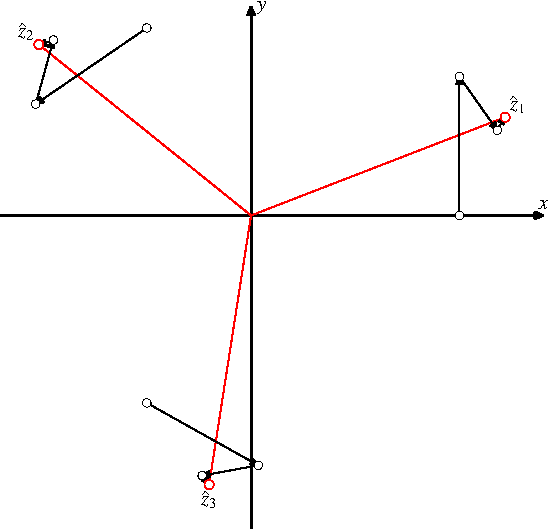
\includegraphics{chapters/images/randwert-3.pdf}
\caption{Drei verschiedene Wurzeln der komplexen Gleichung $z^3=1+2i$
gefunden mit dem Newtonverfahren f"ur drei verschiedene Startpunkte
\label{newton:2dgraphik}}
\end{figure}
